\documentclass[11pt,a4paper]{article}

\usepackage[top=2.4cm,bottom=2.4cm,left=2.6cm,right=2.6cm]{geometry}
\usepackage{amsmath,amssymb,amsthm}
\usepackage{mathtools}
\usepackage{booktabs}
\usepackage[expansion=false]{microtype}
\usepackage{enumitem}
\usepackage[font=small]{caption}
\usepackage{xcolor}
\usepackage[colorlinks=true,linkcolor=blue!45!black,citecolor=blue!45!black,urlcolor=blue]{hyperref}
\usepackage[giveninits=true,maxbibnames=10,url=false,isbn=false]{biblatex}
\addbibresource{references.bib}

\theoremstyle{plain}
\newtheorem{proposition}{Proposition}[section]
\newtheorem{lemma}[proposition]{Lemma}
\newtheorem{corollary}[proposition]{Corollary}
\theoremstyle{definition}
\newtheorem{definition}[proposition]{Definition}
\theoremstyle{remark}
\newtheorem{remark}[proposition]{Remark}

\newcommand{\dd}{\mathrm{d}}
\newcommand{\Var}{\operatorname{Var}}
\newcommand{\Cov}{\operatorname{Cov}}
\newcommand{\Corr}{\operatorname{Corr}}
\newcommand{\Ai}{\operatorname{Ai}}
\newcommand{\Bi}{\operatorname{Bi}}
\newcommand{\E}{\mathbb{E}}
\DeclareMathOperator*{\argmax}{\arg\,max}
\DeclareMathOperator*{\argmin}{\arg\,min}
\newcommand{\Exp}{\operatorname{Exp}}
\newcommand{\Tw}{T_{\mathrm{w}}}
\newcommand{\xpb}{x_{\mathrm{pb}}}
\newcommand{\taupb}{\tau_{\mathrm{pb}}}

% Corrections to previously written text are typeset in red.
\newcommand{\edit}[1]{\textcolor{red}{#1}}

\title{Forecasting tipping times from data: a practical guide}
\author{}
\date{}

\begin{document}
\maketitle
\vspace{-1.1cm}

\begin{abstract}\noindent
        Combining recent results in nonautonomous dynamics and statistical estimation for stochastic differential equations we derive a fully data-driven pipeline for the accurate forecast of tipping times in complex systems.
\end{abstract}

\section{Introduction}\label{sec:intro}
We are concerned with the problem of forecasting the time at which complex systems will undergo critical transitions given past and present data.
The forecast is a (linear) extrapolation of the estimated return rate of nonlinear systems slowly ramped towards a saddle-node bifurcation.
In \S\ref{sec:tipping} we introduce the mathematical formalism of tipping times in slow-fast stochastic processes.
In \S\ref{sec:formulation} we formulate the extrapolation problem and present three techniques to estimate the return rate of a given sample, two of which have already been proposed in the literature and a new one which we introduce.
In \S\ref{sec:observation} we derive a series of conditions that allow for the accurate forecast of the tipping times to be considered when applying this methodology to collected measurements or experiments data.
In \S\ref{sec:application} we apply the forecasting methodology and the observation protocols of \S\ref{sec:formulation} and \S\ref{sec:observation} to simulated and real-world timeseries data.
In \S\ref{sec:conclusion} we conclude.

\section{Tipping time of a slowly ramped systems}\label{sec:tipping}
The prototypical case of critical transitions in complex system is that of a dynamic saddle-node normal form, with slow (linear) passage through the bifurcation and (additive) noisy fluctuations modelled as an It\^o stochastic differential equation of the form
%
\begin{equation}\label{eq:model}
\dd X_t=f\bigl(X_t,\mu(t)\bigr)\,\dd t+\sigma\,\dd W_t,
\qquad
f(x,\mu):=-\mu-x^2,
\qquad
\mu(t):=\mu_0+\varepsilon t ,
\end{equation}
%
where $X_t\in\mathbb R$ is the state of the system, perturbed by a Wiener process $W_t$ with noise amplitude $\sigma>0$, and $\mu(t)$ is the bifurcation parameter, ramped with constant speed $\varepsilon>0$ from an initial value $\mu_0<0$.
The drift term $f(x,\mu)$ in \eqref{eq:model} has two equilibria $x_{\pm}(\mu)=\pm\sqrt{-\mu}$ for any $\mu<0$; at $\mu=0$ the two branches collide $x_+(0)=x_-(0)=0$ in a saddle-node bifurcation and for $\mu>0$ they annihilate each other.
Noisy perturbations around the stable equilibrium $x_+(\mu)$ decay exponentially fast at a rate dictated by the leading eigenvalue of the linearized vector field
%
\begin{equation}\label{eq:eigenvalue}
        \lambda(\mu)\coloneqq\partial_xf(x_+(\mu),\mu)=-2\sqrt{-\mu}<0 , \quad \mu<0 .
\end{equation}
%
Specifically, the quantity $1/|\lambda|$ identifies the \emph{correlation} or \emph{relaxation time} of noisy fluctuations towards $x_+(\mu)$.
Evidently, $|\lambda|\downarrow0$ as $\mu\uparrow0$, which in turn gives asymptotically longer relaxation time and eventually the blow-up $1/|\lambda|\to\infty$; this phenomenon is known as \emph{critical slowing down}.
This behaviour is generic for any complex system close enough to a saddle-node bifurcation as the nonlinear dynamics is reduced to the normal form \eqref{eq:model} by a smooth change in coordinates.

For a given ramp speed $\varepsilon>0$, the time at which the leading eigenvalue \eqref{eq:eigenvalue} vanishes corresponds to the time at which the forcing parameter $\mu(t)$ reaches the saddle-node bifurcation $\mu(t)=0$, which is $\tau\coloneqq-\mu_0/\varepsilon>0$.
Notice that one can rewrite the linear ramp of the forcing parameter to be independent of the initial condition $\mu_0<0$ and parametrized by the time horizon $\tau$ at which the saddle-node bifurcation is reached, i.e.
%
\begin{equation}\label{eq:breaking_time}
        \mu(t) = \mu_0 + \varepsilon t = \varepsilon(t-\tau)<0\quad\forall t<\tau .
\end{equation}
%
Substituting \eqref{eq:breaking_time} in \eqref{eq:eigenvalue} gives us an explicit time dependence of the approach to the saddle-node bifurcation
%
\begin{equation}\label{eq:eigenvalue_time}
        \lambda(t) = -2\sqrt{\varepsilon(\tau-t)}\uparrow0 ,\quad t\uparrow\tau .
\end{equation}

\subsection{Deterministic tipping time}\label{subsec:delay}
Let us first consider the deterministic limit $\sigma\downarrow0$ for which the nonautonomous system \eqref{eq:model} is known as the \emph{dynamic} saddle-node normal form \cite{Berglund2006}.
The time horizon $\tau$ (henceforth \emph{breaking time}) identifies the loss of hyperbolicity of the stable equilibrium branch $x_+(t)\coloneqq x_+(\mu(t))$ as per \eqref{eq:eigenvalue_time}.
In the nonautonomous regime however, the classic notion of $x_+(t)$ is replaced by the pullback attractor $\xpb(t)$ which is the unique solution of \eqref{eq:model} (in the absence of noise $\sigma=0$) satisfying 
%
\begin{equation}\label{eq:pb_attractor}
        \lim_{t\to-\infty}|\xpb(t)-x_+(\mu(t))|=0 .
\end{equation}
%
For a slow passage through the saddle-node bifurcation, i.e. $0<\varepsilon\ll1$, provided that $\mu_0=\lim_{t\to-\infty}\mu(t)\ll0$, the pullback attractor converges to a slow manifold \cite[Thm.~$2.1.7$]{Berglund2006}, which tracks the stable equilibrium branch $x_+(\mu(t))$.
Specifically, the $\xpb(t)$ solution of \eqref{eq:model} lags behind the drift of the \emph{quasi-stationary equilibrium} $x_+(t)$ and persists past the breaking time $\tau$ for some time before blowing-up to $-\infty$.
The trajectory of a slow passage through a saddle-node will thus undergo a bifurcation-induced critical transition at a delayed time $\taupb>\tau$ (henceforth \emph{tipping time}), creating a window of opportunity $\Delta\tau\coloneqq\tau_{\mathrm{pb}}-\tau>0$ to reverse the forcing $\varepsilon$ and avoid the catastrophic dynamical saddle-node.
To quantify the tipping time, and thus identify the window of opportunity, we follow the procedure outlined in \cite{Li2019}.
We start by writing the dynamic saddle-node normal form as a Riccati equation
%
\begin{equation}\label{eq:riccati}
        \frac{\dd x}{\dd t} = f(x,\mu(t)) = \sum_{k=0}^{2}c_k(t)x^k,
\end{equation}
%
with $c_0(t)=\varepsilon(\tau - t)$, $c_1(t)=0$ and $c_2(t)=-1$, and convert it into a second-order, linear system via change of variables $x\mapsto -(c_2(t)y)^{-1}(\dd y/\dd t)$
%
\begin{equation}\label{eq:converted}
        \frac{\dd^2y}{\dd t^2} = c_0(t)y.
\end{equation}
%
Eq.~\eqref{eq:converted} becomes Airy equation in the rescaled time $s\coloneqq \varepsilon^{1/3}(\tau -t)$
%
\begin{equation}\label{eq:airy}
        \frac{\dd^2y}{\dd s^2} = sy,
\end{equation}
%
whose general solution is a linear combination of Airy functions of the first $\Ai(s)$ and second kind $\Bi(s)$ \cite[\S~$10.4$]{Abramowitz1965}.
By backward substitution, and in the past limit $t\to-\infty$, the pullback attractor solving \eqref{eq:riccati} is given by
%
\begin{equation}\label{eq:pullback_attractor}
        x_{\mathrm{pb}}(s) = -\varepsilon^{1/3}\frac{1}{\Ai(s)}\frac{\dd\Ai}{\dd s} .
\end{equation}
%
From \eqref{eq:pullback_attractor}, $x_{\mathrm{pb}}\to-\infty$ as $\Ai\to0$, which occurs at $s\approx2.338$.
It follows trivially that the tipping time of the pullback attractor is given by $\taupb \approx \tau + 2.338\,\varepsilon^{-1/3}$ and thus the opportunity window scales with the reciprocal of the cubic root of the parameter speed, i.e. $\Delta\tau\propto\varepsilon^{-1/3}$.

\subsection{Tipping time distribution}\label{subsec:exit}
We now consider the more general case of stochastic fluctuations of slow passage through the bifurcation by restoring $\sigma>0$ in \eqref{eq:model}.
As a result, the tipping time $\tau_{\mathrm{pb}}$ is treated as a random variable $\tau_{\mathrm{tip}}$ with an associated probability distribution. 
To characterize $\tau_{\mathrm{pb}}$ for general model of slow-fast stochastic saddle-node normal form we follow the procedures outlined in \cite{Miller2012,Herbert2017}.
To start, consider again the singular limit $\varepsilon\downarrow0$ of \eqref{eq:model}, written as a gradient system 
%
\begin{equation}\label{eq:gradient}
        \dd X_t=-V'\bigl(X_t,\mu\bigr)\,\dd t+\sqrt{2D}\,\dd W_t,
        \qquad
        V(x,\mu):=\mu x + \frac{x^3}{3},    
\end{equation}
%
where $V(x,\mu)$ is the potential of the vector field $f(x,\mu)$ and $D\coloneqq\sigma^2/2$ is the diffusion intensity.
The equilibria $x_{\pm}(\mu)=\pm\sqrt{-\mu}$ of $f$ correspond to the stationary points of $V$, respectively its local minimum and local maximum.
At any $\mu<0$, the potential barrier, separating the local minimum $x_+(\mu)$ from the local maximum $x_-(\mu)$ is
%
\begin{equation}\label{eq:barrier}
        \Delta V\coloneqq V\bigl(x_-(\mu)\bigr)-V\bigl(x_+(\mu)\bigr) = \frac43(-\mu)^{3/2} .
\end{equation}
%
The critical transition of a solution of \eqref{eq:model}, starting in a neighbourhood of $x_+(\mu)$, can thus be reframed as the escape of an overdamped particle across the potential barrier $\Delta V$ driven by noisy fluctuations of intensity $D$.
For fixed values of $\mu<0$ such that $\Delta V\gg D$, these escapes are rare events described by Freidlin--Wentzell theory \cite{Freidlin2012} with connections in statistical mechanics \cite{Santolin2025}.
In particular, the event of a trajectory $X_t$ of \eqref{eq:gradient}, starting near $x_+(\mu)$ and reaching $x_-(\mu)$ across the potential barrier $\Delta V$, satisfies a so-called \emph{large deviation principle}.
The \emph{first exit time} of such event \cite[\S~$5.5$]{Gardiner2009}  
%
\begin{equation}\label{eq:first_exit}
        \tau_{\mathrm{exit}} \coloneqq \inf\{t\ge0\;:\;X_t\le x_-(\mu)\}, 
\end{equation}
%
is asymptotically exponentially distributed \cite[Thm.~$2.3$]{Berglund2013}
%
\begin{equation}\label{eq:large_deviation_principle}
        \tau_{\mathrm{exit}}\overset{d}{\approx}\Exp\bigl(k(\mu)\bigr) , \quad D\downarrow0,
\end{equation}
%
where the rate parameter is given by Kramers formula
%
\begin{equation}\label{eq:rate}
        k(\mu)=\frac{\sqrt{V''\bigl(x_+(\mu)\bigr)\,|V''\bigl(x_-(\mu)\bigr)|}}{2\pi}\,\exp\biggl(-\frac{\Delta V}{D}\biggr)
        =\frac{\sqrt{-\mu}}{\pi}\exp\biggl(-\frac{4(-\mu)^{3/2}}{3D}\biggr).
\end{equation}
%
Notice that the reciprocal of the escape rate in \eqref{eq:rate} gives the \emph{mean first exit time} of \eqref{eq:first_exit}, i.e. $\E[\tau_{\mathrm{exit}}] = 1/k(\mu)$.
This result, originally formulated for stationary diffusion \cite{Day1983} and jump processes \cite{Imkeller2006}, was then extended to the dynamic saddle-node normal form \eqref{eq:model}.
Remarkably, the distribution of the tipping time $\tau_{\mathrm{tip}}$ for the slow passage through the bifurcation is greatly dependent by the competing effects of the noise intensity $D$ and the ramp speed $\varepsilon$.
In the limiting regime $D\ll\varepsilon/2$, it was shown that the escapes occur after the breaking time $\tau$.
In particular, the approximate tipping time distribution $\tau_{\mathrm{tip}}\overset{d}{\approx}p_1$, derived in \cite[Eq.~$(19)$]{Miller2012}, reads
%
\begin{equation}\label{eq:small_noise}
        p_1(t)\coloneqq\frac{\varepsilon^{2/3}}{\sqrt{4\pi^{5}D}\,\Bi^{2}\bigl(-\mu(t)\varepsilon^{-2/3}\bigr)\,\mathcal J(t)^{1/2}}
        \exp\Biggl[-\frac{\varepsilon^{2/3}\,\Ai^{2}\bigl(-\mu(t)\varepsilon^{-2/3}\bigr)}
        {4\pi^{2}D\,\Bi^{2}\bigl(-\mu(t)\varepsilon^{-2/3}\bigr)\,\mathcal J(t)}\Biggr] ,
\end{equation}
%
with $\mathcal J(t)\coloneqq\int_{-\infty}^{t}\Ai^{4}\bigl(-\mu(s)\varepsilon^{-2/3}\bigr)\,\dd s$, has support in the interval $\tau+1.17 \varepsilon^{-1/3} < t < \tau + 3.27 \varepsilon^{-1/3}$.
Notice that such interval contains the tipping time of the pullback attractor $\tau_{\mathrm{pb}}\approx\tau+2.338\,\varepsilon^{-1/3}$.
Remarkably, \eqref{eq:small_noise} is approximately Gaussian locally to its maximum
%
\begin{equation}\label{eq:small_noise_approximation}
        \tau_{\mathrm{tip}}\overset{d}{\approx}\mathcal{N}\biggl(\tau_{\mathrm{pb}}\bigl[1+O(D/\varepsilon)\bigr],O\bigl(D\varepsilon^{-5/3}\bigr)\biggr).
\end{equation}
%
In the opposite regime of large noise intensity $\varepsilon/2\ll D$, and up to $-\mu(t)\gg D^{2/3}$, it was later shown that the approximate tipping time distribution $\tau_{\mathrm{tip}}\overset{d}{\approx}p_2$ has a maximum before the breaking time $\tau$ and has the form \cite[Eq.~$(4)$]{Herbert2017}
%
\begin{equation}\label{eq:large_noise}
        p_2(t)\coloneqq k\bigl(\mu(t)\bigr)\,
        \exp\biggl[-\frac{D}{2\pi\varepsilon}\,
        \exp\biggl(-\frac{\Delta V\bigl(\mu(t)\bigr)}{D}\biggr)\biggr] ,
\end{equation}
%
where $k(\mu(t))$ is the Kramers escape rate given in \eqref{eq:rate} and $\Delta V(\mu(t))$ is the potential barrier given in \eqref{eq:barrier}.

\begin{figure}[t]
    \centering 
    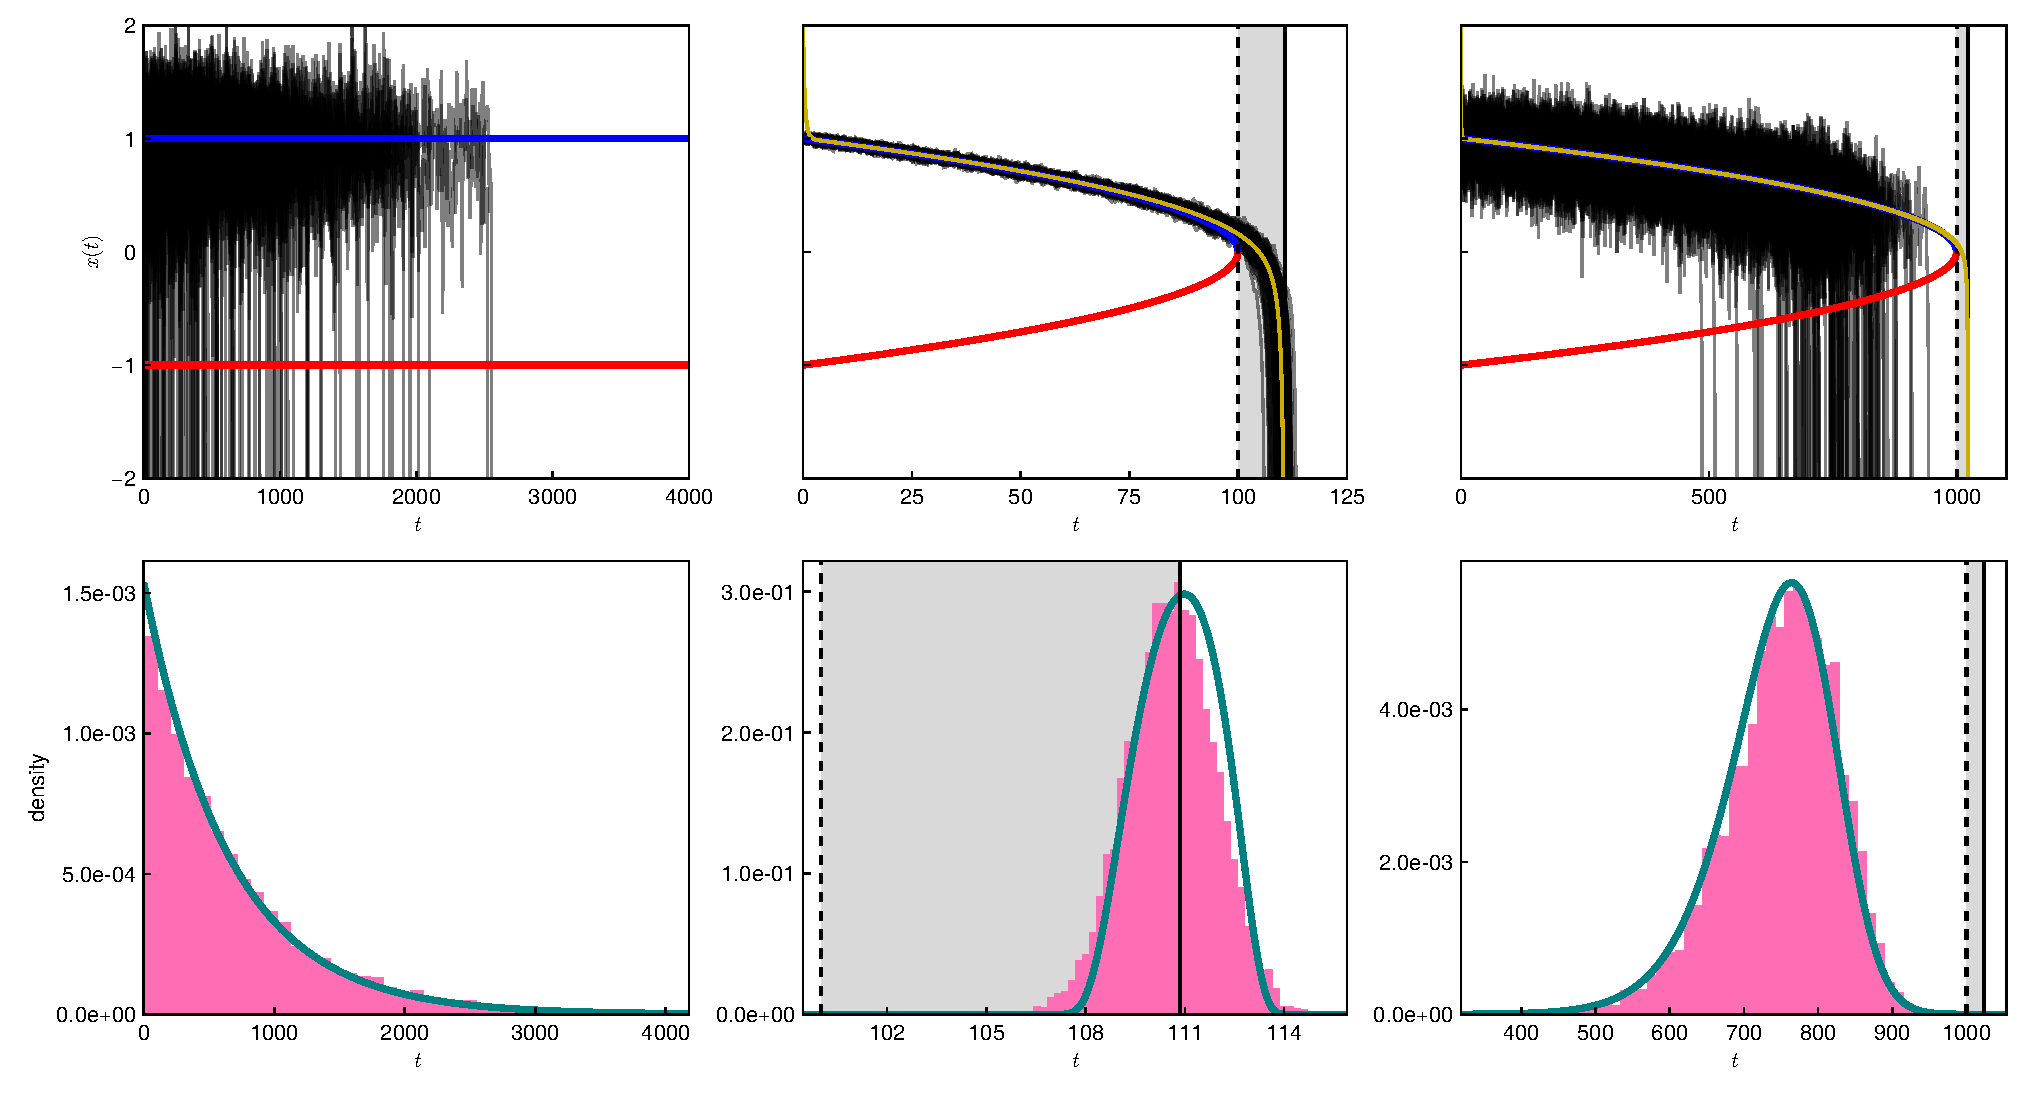
\includegraphics[keepaspectratio, width=\textwidth]{./figures/tipping_times_distribution.pdf}
    \caption{Analytical (teal curves, bottom row) and empirical (pink histograms, bottom row) distribution of the tipping time random variable $\tau_{\mathrm{tip}}$ of $10{,}000$ solutions (black curves, top row) of the saddle-node normal form \eqref{eq:model} from the stable branch $x_+(\mu(t))$ (blue curves, top row) across the unstable branch $x_-(\mu(t))$ (red curves, top row).
             Leftmost column (N-tipping): stationary regime \eqref{eq:large_deviation_principle} with $\mu=-1$ and $D=0.25$.
             Middle column (B-tipping): slow passage through the bifurcation \eqref{eq:small_noise} with $\mu_0=-1$, $\varepsilon=10^{-2}$ and $D=10^{-3}$.
             Rightmost column (N-tipping): early escapes due to large noise \eqref{eq:large_noise} with $\mu_0=-1$, $\varepsilon=10^{-3}$ and $D=0.06$.
             The window of opportunity $\Delta\tau$ (gray shaded band in the middle and rightmost columns) is bounded from below (dashed black lines) by the breaking time $\tau$ and from above (solid black lines) by the tipping time of the pullback attractor $\tau_{\mathrm{pb}}$ (orange curve, top row).
     }
    \label{fig:tipping_times_distribution}
\end{figure}

\section{Forecasting problem}\label{sec:formulation}
From \S\ref{sec:tipping}, we summarize three important results that motivate the forecasting of tipping times:
%
\begin{enumerate}
        \item for a slow passage through a saddle-node bifurcation the leading eigenvalue $\lambda(t)$ explicitly depends on the breaking time $\tau$ via Eq.~\eqref{eq:eigenvalue_time};
        \item the time at which a slowly ramped solution tips $\tau_{\mathrm{pb}}$ is delayed with respect to the breaking time $\tau$ by a factor of $\varepsilon^{-1/3}$ that depends on the speed of the forcing, thereby creating an opportunity window $\Delta\tau$;
        \item in the small noise regime $\sigma=\sqrt{2D}\ll\sqrt{\varepsilon}$, the delayed tipping time of a noisy solution $\tau_{\mathrm{tip}}$ occurs almost always after the breaking time $\tau$, as per the support of the density $p_1(t)$ in Eq.~\eqref{eq:small_noise}, and on average close to the deterministic tipping time, i.e. $\E[\tau_{\mathrm{tip}}]\approx\tau_{\mathrm{pb}}$ as per Eq.~\eqref{eq:small_noise_approximation}.
\end{enumerate}
%
Provided a timeseries that is slowly ramped towards a saddle-node bifurcation, with noise and speed satisftying $0<\sigma^2\ll\varepsilon\ll1$, then, if we accurately forecast the breaking time $\tau$ (by $1.$), we can avoid the bifurcation-induced catastrophe with high probability (by $3.$) by reversing the forcing $\varepsilon$ within a time window $\Delta\tau>0$ (by $2.$).
To formulate the forecasting problem of the breaking time $\tau$ we introduce the \emph{(squared) return rate} $\alpha(t)\coloneqq\lambda^2(t)$, where $\lambda(t)$ is given in \eqref{eq:eigenvalue_time}
%
\begin{equation}\label{eq:return_rate}
        \alpha(t) = 4\varepsilon(\tau-t)>0\quad\forall t<\tau . 
\end{equation}
%
Notice that, while $\alpha(t)\downarrow0$ as $t\uparrow\tau$ just like $-\lambda(t)$ does in \eqref{eq:eigenvalue_time}, Eq.~\eqref{eq:return_rate} establishes an affine dependence of the return rate on time $t$.
This property benefits the forecasting of $\tau$ using timeseries data that preceede the critical transition.
To understand this suppose that $\mathcal{X}\coloneqq\{X_j\coloneqq X_{t_j}\}_{j=1,\dots,n}$ is a solution of \eqref{eq:model} with $t_j<t_{j+1}$, that is in a regime of safe distance from the bifurcation, i.e. $t_n\ll\tau$.
Assuming we are able of doing so, we can estimate the true return rate \eqref{eq:return_rate} from the sample $\mathcal{X}$, thus yielding a sequence $\hat{\alpha}\coloneqq\{\hat\alpha_j\coloneqq\hat\alpha(t_j)\}_{j=1,\dots,n}$.
Given the estimate sequence $\hat\alpha$, we can fit a linear model of the form $\hat\alpha(t) = \hat m t + \hat q$, with slope $\hat m$ and offest $\hat q$. 
Then, the forecasted breaking time $\hat\tau$ corresponds to the zero-crossing of the linear fit, which, by extrapolation, reads $\hat\tau = -\hat q/\hat m$.
Consequally, we translated the problem of forecasting the breaking time $\tau$ from timeseries data $\mathcal{X}$ into a trivial, linear extrapolation $\hat\tau$ from estimates $\hat\alpha$.
Clearly, this problem features two bottlenecks for the accuracy of the forecasted $\hat\tau$: first, we need the estimates $\hat\alpha$  to be as close as possible to the ground truth $\alpha$ and; second, given those estimates $\hat\alpha$, we need the linear extrapolation $\hat\tau=-\hat q/\hat m$ to be as close as possible to the ground truth $\tau$.
In particular, depending on applications, we would prefer to slightly underestimate the breaking time $\hat\tau\lesssim\tau$, rather than slightly overestimating it $\hat\tau\gtrsim\tau$, thereby biasing our forecast to minimize missed allarms (i.e. false negatives) in favour of spurious warnings (i.e. false positives).
In the remaining of this section we present three data-driven techniques to accurately extract the estimates $\hat\alpha$ from a sample $\mathcal{X}$ while we address the problem of precise extrapolation in \S\ref{sec:observation}.

\subsection{Ornstein-Uhlenbeck approximation}\label{subsec:OUP}
Let us start by characterising the statistical properties of the noisy fluctuations of a solution $\mathcal{X}$ of \eqref{eq:model} around the pullback attractor $x_{\mathrm{pb}}(t)$ given in Eq.~\eqref{eq:pullback_attractor}.
We write the solution variable as a superposition $X_t\coloneqq x_{\mathrm{pb}}(t)+Z_t$ of a determistic $x_{\mathrm{pb}}(t)$ and a stochastic component $Z_t$.
Substituting this into \eqref{eq:model}, recalling that by definition $\dd\xpb=f(\xpb,\mu)\dd t$, we get
%
\begin{equation}\label{eq:fluctuations}
        \dd Z_t=\bigl(-2\xpb(t)\,Z_t-Z_t^2\bigr)\dd t+\sigma\,\dd W_t .
\end{equation}
%
Let us consider time instances $t\ll\tau$ away from the saddle-node bifurcation; in this case $f(\xpb,\mu)\approx f\bigl(x_+(\mu),\mu\bigr)$ which implies $\partial_x f(\xpb,\mu)\approx\lambda(t)$.
Subsituting this into \eqref{eq:fluctuations} gives
%
\begin{equation}\label{eq:fluctuations_scaled}
        \dd Z_t=\bigl(\lambda(t)\,Z_t-Z_t^2\bigr)\dd t+\sigma\,\dd W_t .
\end{equation}
%
It can be shown that $|Z_t|\approx\sigma/\sqrt{2|\lambda(t)|}$ \cite[Thm.~$4.1$]{Kuehn2011}, and thus $Z_t^2=o(|\lambda(t)Z_t|)$ for any $\sigma\ll\sqrt{\varepsilon}$ and any time $t\ll\tau$ such that $\sigma\ll\sqrt{2}\bigl(4\varepsilon(\tau-t)\bigr)^{3/4}$.
We can therefore reasonably approximate \eqref{eq:fluctuations_scaled} by neglecting the nonlinear term $Z_t^2$, thereby obtaining 
%
\begin{equation}\label{eq:oup}
        \dd Z_t\approx\lambda(t)\,Z_t\dd t+\sigma\,\dd W_t .
\end{equation}
%
The linear, nonautonomous Eq.~\eqref{eq:oup} is a time-inhomogeneous Ornstein-Uhlenbeck process.
Suppose the sample $\mathcal{X}$ is recorded across a time window $T_w>0$ in which the underlying forcing parameter $\mu(t)$ changes very little, i.e.
%
\begin{equation}\label{eq:sample_assumption}
        \mathcal{X}=\{X_{t_j}\}_{j=1,\dots,n} , \quad \text{such that} \quad |\mu(t_1)-\mu(t_n)|\approx0.
\end{equation}
%
Then $\lambda(t)\approx\lambda$ is approximately constant and \eqref{eq:oup} admits a stationary solution \cite[\S~$3.8$]{Gardiner2009} with zero mean $\E[Z_t]\eqqcolon\bar{Z}=0$ and variance $\Var[Z_t]\eqqcolon\gamma=\sigma^2/2|\lambda|$.
Written in terms of the return rate $\alpha=\lambda^2$, the last identity reads
%
\begin{equation}\label{eq:oup_variance}
        \gamma = \frac{\sigma^2}{2\sqrt{\alpha}} .
\end{equation}
%
Let $\hat\gamma$ be the sample variance of $\mathcal{X}$, then \eqref{eq:oup_variance} gives a sample estimate of the return rate
 
\begin{equation}\label{eq:OUP}
        \hat\alpha = \frac{\sigma^4}{4\hat\gamma^2} .
\end{equation}

\subsection{Autoregressive approximation}\label{subsec:AC1}
In the same time window $T_w>0$ above, the homogeneous Ornstein-Uhlenbeck process has correlation function $\Corr(Y_t,Y_{t+Tw})=\gamma\exp\bigl(-\sqrt{\alpha}T_w\bigr)$ \cite[\S~$3.8$]{Gardiner2009}, with $\gamma$ given in \eqref{eq:oup_variance}.
As a result, the discrete observations in sample $\mathcal{X}$ can be approximated by fitting a continuous-time autoregressive model of order one
%
\begin{equation}\label{eq:autoregressive}
        X_{j+1}\approx\rho X_{j} + \sqrt{\gamma(1-\rho^2)}\,\eta_t , \quad \eta_t\sim\mathcal{N}(0,1),
\end{equation}
%
where 
%
\begin{equation}\label{eq:ac1}
        \rho\coloneqq\gamma^{-1}\Corr(X_t,X_{t+\Delta}), \quad \Delta=t_{j+1}-t_j, 
\end{equation}
%
is the autocorrelation coefficient at lag$-1$.
Given the sample mean $\hat X$ the sample autocorrelation coefficient can be obtained by maximum likelihood estimation
%
\begin{equation}\label{eq:ac1_sample}
        \hat\rho = \frac{\sum_{j=1}^{n-1}(X_j - \hat X)(X_{j+1} - \hat X)}{\sum_{j=1}^{n}(X_j - \hat X)^2}.
\end{equation}
%
Using \eqref{eq:ac1_sample} one can estimate the return rate of the sample $\mathcal{X}$ using the autoregressive approximation 
%
\begin{equation}\label{eq:AC1}
        \hat\alpha = \biggl(\frac{\log\hat\rho}{\Delta}\biggr)^2.
\end{equation}
%
Autoregressive based early-warning signals have found widespread applications in ecology \cite{Dakos2012} and climate science \cite{Boers2021}.
In particular, estimators of the form \eqref{eq:AC1} have been used in \cite{Ditlevsen2023} for estimating the tipping time of the subpolar gyre of the Atlantic Meridional Overturning Circulation system and in \cite{Ashwin2025} for establishing a framework that quantifies the predicting skill of early-warning signals.

\subsection{Euler-Maruyama approximation}\label{subsec:LLS}
A solution of the nonlinear system \eqref{eq:model} in a time window $T_w>0$ as per above, can be approximated by the process \cite[\S~$8.4$]{Lord2014}
%
\begin{equation}\label{eq:EM}
        X_{t+1} = X_t + f(X_t,\mu)\Delta + \sigma\sqrt{\Delta}\,\eta_t , \quad \eta_t\sim\mathcal{N}(0,1) .
\end{equation}
%
The sequence above is the Euler-Maruyama approximation of \eqref{eq:model} and it corresponds to the stochastic generalization of the Euler time-stepping method for ordinary differential equations.
We can rearrange the terms in \eqref{eq:EM} to define the first-order time increments of the Euler-Maruyama approximation
%
\begin{equation}\label{eq:increments}
        Y_t\coloneqq\frac{X_{t+1} - X_t}{\Delta} = f(X_t,\mu) + \tilde{\eta}_t , \quad \tilde{\eta}_t\sim\mathcal{N}\biggl(0,\frac{\sigma^2}{\Delta}\,\biggr) .
\end{equation}
%
Provided a sample $\mathcal{X} = \{X_j\}_{j=1,\dots,n}$ in a time window $T_w=n\Delta$, and a choice of the model function $f$, Eq.~\eqref{eq:increments} can be interpreted as a ordinary least square regression problem, with the residuals $r_j\coloneqq Y_{j+1} - f(X_j)=\tilde{\eta}_t$ being normally distributed.
Away from the saddle-node bifurcation, the sample is approximately an Ornstein-Uhlenbeck process of the form \eqref{eq:oup} and thus we can reasonably fit a linear model of the form $f(x,\theta) = \theta_0 + \theta_1 x$ to the time increments $Y_j$.
Substituting this ansatz into \eqref{eq:increments}, and minimizing the square root of the sum of the squared residuals across the sample, yields the ordinary least square problem
%
\begin{equation}\label{eq:ordinary_least_squares}
        \hat\theta = \argmin_{\theta\in\mathbb{R}^2}\Biggl(\sqrt{\sum_{j=1}^{n-1}\bigl(Y_j-f(X_j,\theta)\bigr)^2}\Biggr) , \quad \hat{\theta} = \Bigl(\hat{\theta}_0, \hat{\theta}_1\Bigr)^T.
\end{equation}
%
Notice that $f\in\mathbb{P}_1[x]$, meaning that the problem \eqref{eq:ordinary_least_squares} is linear in $\theta$; the solution of the ordinary (linear) least squares problem is thus found by the normal equation
%
\begin{equation}\label{eq:normal_equation}
        \hat\theta = (A^TA)^{-1}A^TY,
\end{equation}
%
where $Y=(Y_j)_{j=1,\dots,n-1}$ is the vector of observed time increments of the sample $\mathcal{X}$ and $A=(1, X_j)_{j=1,\dots,n-1}$ is the model matrix of the linear fit $f$ to the sample $\mathcal{X}$.
Notice that, by definition, $\hat{\theta}_1$ is an estimate of the leading eigenvalue $\lambda$ of the underlying nonlinear evolution and thus
%
\begin{equation}\label{eq:LLS}
        \hat\alpha = \hat{\theta}_1^{\,2},
\end{equation}
%
is a sample estimate of the return rate using an ordinary linear least square approximation. 

\section{Observation protocol}\label{sec:observation}
The return rate estimators using the Ornstein-Uhlenbeck \eqref{eq:OUP}, autoregressive \eqref{eq:AC1} and linear least squares \eqref{eq:LLS} approximations all provide a data-drive pipeline to extract $\hat\alpha$ from a given sample $\mathcal{X}$ collected over a time window $T_w=n\Delta$, with $n>0$ number of observations sampled at (regular) frequency $\Delta$.
As noted at the beginning of \S~\ref{sec:formulation} however, these estimates are only useful to forecast the tipping time $\hat\tau$ of the given sample $\mathcal{X}$.
In this section we address this problem in two parts. 
First, we discuss the uncertainties in the return rate estimators $\hat\alpha$ derived above induced by finite samples: in particular we introduce the rolling window technique and derive a data-driven protocol for the optimal collection of observations that minimize the bias and uncertainty in the estimation of the return rate.
Second, we formulate the extrapolation problem of $\hat\tau$ given a sequence $\hat\alpha=\{\hat\alpha_j\}_{j=1,\dots,n}$ of optimal estimators of the return rate and provide a data-driven pipeline for the accurate forecasting problem.

\subsection{Accuracy and precision of the estimators}\label{subsec:estimators}

\subsubsection{Admissible time horizon}\label{subsubsec:horizon}
The analytical return rate \eqref{eq:return_rate}, and thus the sample estimators \eqref{eq:OUP}, \eqref{eq:AC1} and \eqref{eq:LLS}, is obtained from the time-dependent eigenvalue \eqref{eq:eigenvalue_time}, which is itself evaluated along the drifting quasi-steady equilibrium $x_+(\mu(t))$.
However, a sample $\mathcal{X}$ that is a solution of \eqref{eq:model} follows the pullback attractor \eqref{eq:pb_attractor}, which lags behind $x_+(\mu(t))$ at any $t<\tau$.
After a fast relaxation of the initial condition, in the slow regime the distance at which $x_{\mathrm{pb}}(t)$ tracks $x_+(\mu(t))$ increases with time and it reaches its maximum at the saddle-node bifurcation $|x_{\mathrm{pb}}(t)-x_+(\mu(t))|=O(\varepsilon^{1/3})$, $t\uparrow\tau$ \cite[Thm.~$2.2.2$]{Berglund2006}.
We are thus interested to quantify a time horizon $T_c\ll\tau$ for which the return rate $\alpha(t)$ of the quasi-steady equilibrium is accurate, at least to first-order, to that of the pullback attractor $\alpha_{\mathrm{pb}}(t)=\lambda_{\mathrm{pb}}^2(t)=4x_{\mathrm{pb}}^{\,2}(t)$.
Sufficiently far from the saddle-node bifurcation we can exploit the asymptotic expansion of Airy's function \cite[\S~$10.4$]{Abramowitz1965} to approximate \eqref{eq:pullback_attractor} to first-order
%
\begin{equation}\label{eq:asymptotic_pullback_attractor}
  x_{\mathrm{pb}}(s)\approx \varepsilon^{1/3}\biggl(\sqrt{s} + \frac{1}{4s}\biggr) , \quad s=\varepsilon^{1/3}(\tau-t)\to\infty.
\end{equation}
%
In this regime, the return rate for the pullback attractor is thus
%
\begin{equation}\label{eq:pb_return_rate}
  \alpha_{\mathrm{pb}}(t) = \alpha(t) + \frac{1}{4(\tau-t)^2} + 2\sqrt{\frac{\varepsilon}{\tau-t}},
\end{equation}
%
and dividing each term in \eqref{eq:pb_return_rate} by $\alpha(t)$ gives
%
\begin{equation}\label{eq:lag_correction}
  \frac{\alpha_{\mathrm{pb}(t)}}{\alpha(t)} = 1 + \frac{1}{16 \varepsilon(\tau - t)^3} + \frac{1}{2\sqrt{\varepsilon}(\tau - t)^{3/2}} = 1 + 2\eta(t) + \eta^2(t) = \bigl(1+\eta(t)\bigr)^2 ,
\end{equation}
%
where $\eta(t)=1/4\sqrt{\varepsilon}(\tau-t)^{3/2}$.
The admissible time horizon $T_c$ easily follows
%
\begin{equation}\label{eq:admissible_time_horizon}
  T_c = 
\end{equation}

Equation \eqref{eq:pullback_attractor} also settles what the extrapolation targets, without recourse to \eqref{eq:relerr}.
The squared return rate $\alpha_{\mathrm{pb}}=4\xpb^{2}$ vanishes precisely where $\dd\Ai/\dd s$ does, which on the interval between the first zero of $\dd\Ai/\dd s$ and $s\to+\infty$ occurs at the single point $s\approx-1.019$ \cite[\S~$10.4$]{Abramowitz1965}, that is at $t\approx\tau+1.019\,\varepsilon^{-1/3}$.
The squared return rate along the pullback attractor thus reaches zero after the breaking time and before the blow-up at $\taupb$, the two separated by one inner width, where \eqref{eq:relerr} has in any case expired.
The zero-crossing of the fitted line therefore estimates the breaking time $\tau$ of the leading-order law \eqref{eq:return_rate}, and the tipping time must be recovered from it by the delay of \S\ref{subsec:delay},
%
\begin{equation}\label{eq:taupb_hat}
        \hat\tau_{\mathrm{pb}}=\hat\tau+2.338\,\hat\varepsilon^{\,-1/3} .
\end{equation}
%
The ramp speed needed in \eqref{eq:taupb_hat} is supplied by the same fit that produces $\hat\tau$: comparing $\hat\alpha(t)=\hat mt+\hat q$ with \eqref{eq:return_rate} identifies
%
\begin{equation}\label{eq:epshat}
        \hat\varepsilon=-\frac{\hat m}{4} ,
\end{equation}
%
so that no independent knowledge of the forcing is required, and the consistency of the pair $(\hat q,\hat m)$ with $\hat q=-\hat m\hat\tau$ is automatic.

\subsubsection{Finite-sample effects}\label{subsubsec:effects}
% 4.1.2
% 4.1.3
% 4.1.8

\subsubsection{Windowed observation}\label{subsubsec:window}
% 4.1.4
% 4.1.5
% 4.1.6
% 4.1.7

\subsection{Extrapolating the tipping time}\label{subsec:extrapolators}

\section{Practical applications}\label{sec:application}

\section{Conclusions}\label{sec:conclusion}

\printbibliography

\end{document}
